%! Author = Stepan Oskin
%! Date = 11-Jul-19

% Preamble
\documentclass[11pt]{article}

% Packages
\usepackage{amsmath, subcaption}
\usepackage{graphicx}

% New commands
\newcommand{\norm}[1]{\left\lVert#1\right\rVert}
\newcommand{\vect}[1]{\boldsymbol{#1}}
\newcommand{\pa}[1]{\partial{#1}}

% Document
\begin{document}

    \title{Mathematics of the Adaline learning algorithm\\
    Excerpts from Python Machine Learning \\
    Second Edition \\
    By Sebastian Raschka and Vahid Mirjalili\cite{RaschkaMirjalili2017} \\
    and other sources}

    \author{Stepan Oskin}

    \maketitle

    \begin{abstract}


    \end{abstract}

    \section{Introduction} \label{sec:ada_intro}

    \subsection{Classification} \label{subsec:classification}

    Classifying data is a common task in machine learning.
    Suppose some given data points each belong to one of two classes, and the goal is to decide which class a
    new data point will be in.

    In the case of the Adaline learning algorithm, a data point is viewed as a $p$-dimensional vector
    (a list of $p$ numbers), and we want to know whether we can separate such points with
    a $(p-1)$-dimensional hyperplane.
    This is called a linear classifier.
    More formally, we can put the idea behind artificial neurons into the context of a binary classification task where we refer to our two classes as 1 (positive class) and -1 (negative class) for simplicity.
    There are many hyperplanes that might classify the data.
    We can then define a decision function ($\phi(z)$) that takes a linear combination of certain input values $x$ and a corresponding weight vector $w$, where $z$ is the so-called net input.

    \subsection{Adaline learning algorithm for classification} \label{subsec:ada_desc}

    Adaline learning algorithm for classification presents another type of single-layer neural network.
    \textbf{ADAptive LInear NEuron (Adaline)} was published by \textit{Bernard Widrow} and his doctoral student \textit{Tedd Hoff}\cite{Widrow1960}, only a few years after \texitit{Frank Rosenblatt's} perceptron algorithm\cite{Rosenblatt1957a}, and can be considered as an improvement on the latter.

    \subsection{Minimizing continuous cost functions} \label{subsec:min_con_cost}

    The Adaline algorithm is particularly interesting because it illustrates the key concepts of defining and minimizing \textbf{continuous cost functions}.
    This lays the groundwork for understanding more advanced machine learning algorithms for classification, such as logistic regression, support vector machines, and regression models.

    The \textbf{key difference} between the Adaline rule (also known as the \textbf{Widrow-Hoff} rule) and Rosenblatt's perceptron is that the weights are updated based on a \textbf{linear activation function} rather than a unit step function like in the perceptron.
    In Adaline, this linear activation function $\phi(z)$ is simply the \textbf{identity function} of the net input, so that:

    \begin{equation}
        \label{eq:ada_func_act}
        \phi ( \vect{w}^T \vect{x} ) = \vect{w}^T \vect{x}
    \end{equation}

    While the linear activation function is used for learning the weights, we still use a threshold function to make the final prediction, which is similar to the unit step function that was described for the perceptron.
    The main differences between the perceptron and Adaline algorithm are highlighted in figure~\ref{fig:adaline_dag}.

    \begin{figure}[hbt!]
        \centering
        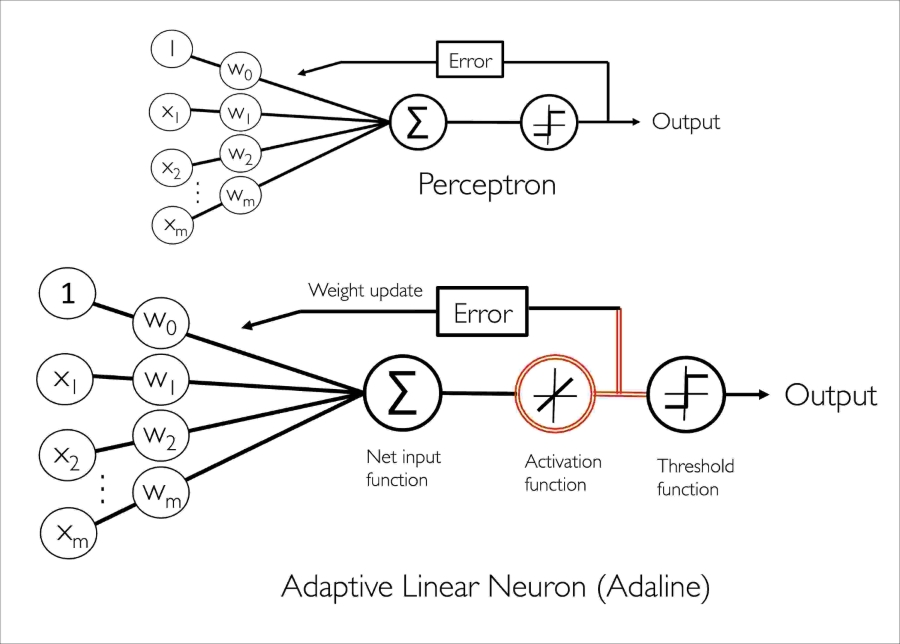
\includegraphics[width=1\linewidth,trim=1 1 1 1,clip]{img/adaline_dag.jpg}
        \caption{Adaline algorithm compares the true class labels with the linear activation function's continuous valued output to compute the model error and update the weights.
        In contrast, the perceptron compares the true class labels to the predicted class labels.}
        \label{fig:adaline_dag}
    \end{figure}

    Figure~\ref{fig:adaline_dag} shows that the Adaline algorithm compares the true class labels with the linear activation function's \textbf{continuous valued output} to compute the model error and update the weights.
    In contrast, the perceptron compares the true class labels to the predicted class labels.

    \section{Minimizing cost functions with gradient descent} \label{sec:ada_grad_desc}

    \subsection{Continuous cost function in Adaline} \label{subsec:ada_cost}

    One of the key ingredients of supervised machine learning algorithms is a defined \textbf{objective function} that is to be optimized during the learning process.
    This objective function is often a cost function that we want to minimize.
    In the case of Adaline, we can define the \textbf{cost function} $J$ to learn the weights as the \textbf{Sum of Squared Errors (SSE)} between the calculated outcome and the true class label:

    \begin{equation}
        \label{eq:ada_func_cost}
        J ( \vect{w} ) = \frac{1} {2} \sum_i \left( y^{(i)} - \phi \left( z^{(i)} \right) \right) ^2
    \end{equation}

    The term $\frac{1} {2}$ is just added for convenience, which will make it easier to derive the gradient, as we will see in the following paragraphs.
    The main advantage of this continuous linear activation function, in contrast to the unit step function, is that the \textbf{cost function becomes differentiable}.
    Another nice property of this cost function is that it is \textvbf{convex}; thus, we can use a simple yet powerful optimization algorithm called \textbf{gradient descent} to find the weights that minimize our cost function to classify the samples in the Iris dataset.

    \subsection{Optimizing convex and continuous functions using Gradient Descent} \label{subsec:grad_desc}

    As illustrated in figure~\ref{fig:grad_desc}, we can describe the main idea behind gradient descent as climbing down a hill until a local or global cost minimum is reached.
    In each iteration, we take a step in the opposite direction of the gradient where the step size is determined by the value of the learning rate, as well as the slope of the gradient:

    \begin{figure}[hbt!]
        \centering
        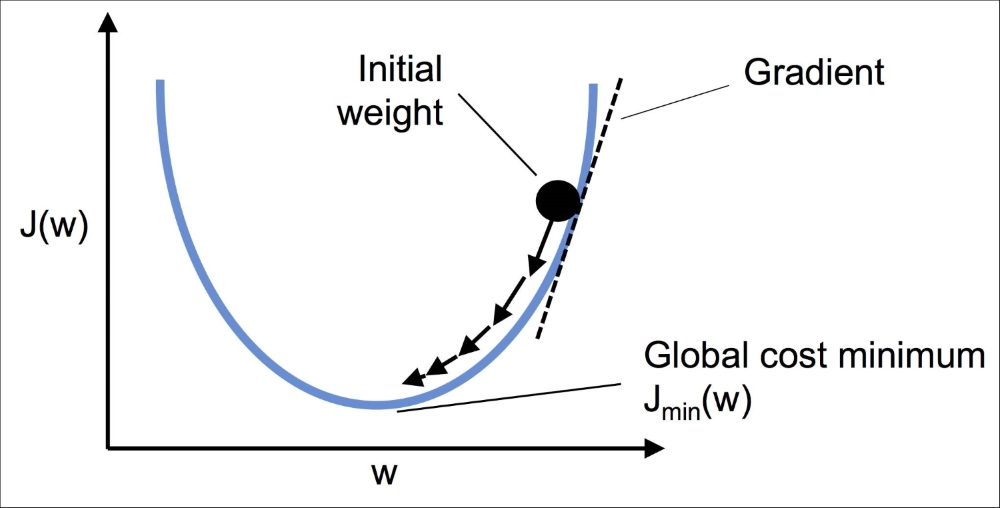
\includegraphics[width=1\linewidth,trim=4 4 4 4,clip]{img/grad_desc.jpg}
        \caption{Main idea behind gradient descent optimization algorithm can be described as climbing down a hill until a local or global cost minimum is reached.
        In each iteration, we take a step in the opposite direction of the gradient where the step size is determined by the value of the learning rate, as well as the slope of the gradient.}
        \label{fig:grad_desc}
    \end{figure}

    Using gradient descent, we can now update the weights by taking a step in the opposite direction of the gradient $\nabla J(w)$ of our cost function:

    \begin{equation}
        \label{eq:weight_update}
        \vect{w} := \vect{w} + \Delta \vect{w}
    \end{equation}

    Where the weight change $\Delta \vect{w}$ is defined as the negative gradient multiplied by the learning rate $\eta$:

    \begin{equation}
        \label{eq:delta_w}
        \Delta \vect{w} = - \eta \nabla J (\vect{w})
    \end{equation}

    \subsection{Computing partial derivatives of the cost function} \label{subsec:ada_grad_pd}

    To compute the gradient of the cost function, we need to compute the partial derivative of the cost function with respect to each weight $w_j$:

    \begin{equation}
        \label{eq:dJ_dw}
        \frac{ \pa{J} } { \pa{w_j} } = - \sum \limits_i \left( y^{(i)} - \phi \left( z^{(i)} \right) \right) x_j^{(i)}
    \end{equation}

    The full derivation can be obtained using the chain rule of differentiation:

    \begin{equation}
        \begin{split}
            \frac{ \pa{J} } { \pa{w_j} } & =
            \frac{\partial} {\pa{w_j}} \frac{1} {2} \sum \limits_i \left( y^{(i)} - \phi \left( z^{(i)} \right) \right) ^2 = \\
            & = \frac{1} {2} \frac{\partial} {\pa{w_j}} \sum \limits_i \left( y^{(i)} - \phi \left( z^{(i)} \right) \right) ^2 = \\
            & = \frac{1} {2} \sum \limits_i 2 \left( y^{(i)} - \phi \left( z^{(i)} \right) \right) \frac{\partial} {\pa{w_j}} \left( y^{(i)} - \phi \left( z^{(i)} \right) \right) = \\
            & = \sum \limits_i \left( y^{(i)} - \phi \left( z^{(i)} \right) \right) \frac{\partial} {\pa{w_j}} \left( y^{(i)} - \sum \limits_i \left( w_j^{(i)} x_j^{(i)} \right) \right) = \\
            & = \sum \limits_i \left( y^{(i)} - \phi \left( z^{(i)} \right) \right) \left( - x_j^{(i)} \right) = \\
            & = -\sum \limits_i \left( y^{(i)} - \phi \left( z^{(i)} \right) \right) x_j^{(i)}
        \end{split}
    \end{equation}

    \section{An object-oriented Adaline API using NumPy} \label{sec:ada_api}

    \subsection{Adaline learning rule} \label{subsec:ada_learn_rule}

    After the partial derivatives of the cost function with respect to weights have been computed, we can re-write the update of weight $w_j$ as:

    \begin{equation}
        \label{eq:ada_weight_update}
        \Delta w_j = - \eta \frac{ \pa{J} } { \pa{w_j} } =
        \eta \sum \limits_i \left( y^{(i)} - \phi \left( z^{(i)} \right) \right) x_j^{(i)}
    \end{equation}

    Since we update all weights simultaneously, our Adaline learning rule becomes:

    \begin{equation}
        \label{eq:ada_learn_rule}
        \boldsymbol{w} := \boldsymbol{w} + \Delta \boldsymbol{w}
    \end{equation}

    Although the Adaline learning rule looks identical to the perceptron rule, we should note that the $\phi \left( z^{(i)} \right)$ with is a real number and not an integer class label.
    Furthermore, the weight update is calculated based on all samples in the training set (instead of updating the weights incrementally after each sample), which is why this approach is also referred to as \textbf{batch gradient descent}.

    \subsection{Description of the implementation} \label{subsec:ada_impl}

    Since the perceptron rule and Adaline are very similar, \textit{Raschka and Mirjalili}\cite{RaschkaMirjalili2017} took the perceptron implementation that was defined earlier and changed the \texttt{fit} method so that the weights are updated by minimizing the cost function via gradient descent.

    Instead of updating the weights after evaluating each individual training sample, as in the perceptron, the gradient is calculated based on the whole training dataset via \texttt{self.eta * errors.sum()} for the bias unit (zero-weight) and via \texttt{self.eta * X.T.dot(errors)} for the weights 1 to m where \texttt{X.T.dot(errors)} is a matrix-vector multiplication between our feature matrix and the error vector.

    Note that the \texttt{activation} method has no effect in the code since it is simply an identity function.
    The \texttt{activation} function (computed via the activation method) was added to illustrate how information flows through a single layer neural network: features from the input data, net input, activation, and output.
    Other classifiers, such as logistic regression, use a non-identity, nonlinear activation function.
    \textbf{Logistic regression} model is closely related to Adaline with the only difference being its activation and cost function.

    Now, similar to the previous perceptron implementation, cost values are collected in a \texttt{self.cost\_} list to check whether the algorithm converged after training.

    \subsection{Selecting the learning rate} \label{subsec:ada_learn_rate}

    In practice, it often requires some experimentation to find a good learning rate $\eta$ for optimal convergence.
    On figure~\ref{fig:ada_learn_rate}, two different learning rates, $\eta=0.1$ and $\eta=0.0001$, were chosen and the cost functions versus the number of epochs were plotted to see how well the Adaline implementation learns from the training data.

    \begin{figure}[hbt!]
        \centering
        \begin{subfigure}[t]{.48\textwidth}
            \centering
            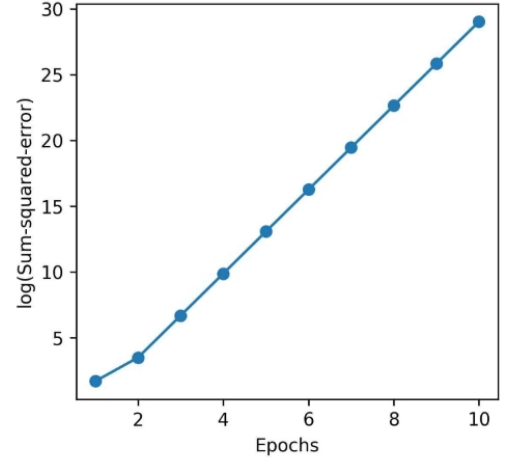
\includegraphics[width=\columnwidth,trim=4 4 4 4,clip]{img/ada_learn_rate_001.png}
            \caption{$\eta=0.01$}
            \label{fig:ada_learn_rate_001}
        \end{subfigure}
        ~ %add desired spacing between images, e. g. ~, \quad, \qquad, \hfill etc.
        %(or a blank line to force the subfigure onto a new line)
        \begin{subfigure}[t]{.48\textwidth}
            \centering
            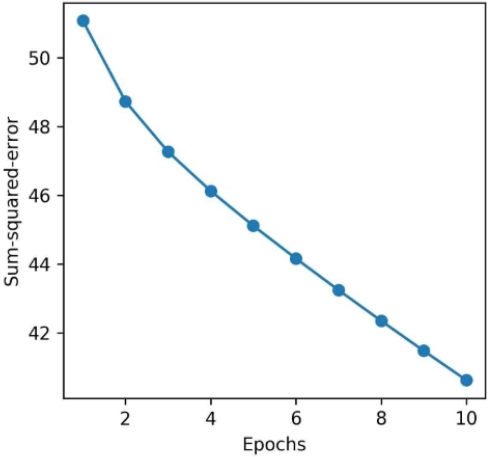
\includegraphics[width=\columnwidth,trim=4 4 4 4,clip]{img/ada_learn_rate_00001.png}
            \caption{$\eta=0.0001$}
            \label{fig:ada_learn_rate_00001}
        \end{subfigure}
        \caption{It often requires some experimentation to find a good learning rate $\eta$ for optimal convergence.
        Two different learning rates, $\eta=0.1$ (\ref{fig:ada_learn_rate_001}) and $\eta=0.0001$(\ref{fig:ada_learn_rate_00001}), were chosen and the cost functions versus the number of epochs were plotted to see how well the Adaline implementation learns from the training data.}
        \label{fig:ada_learn_rate}
    \end{figure}

    The learning rate $\eta$ (\texttt{eta}), as well as the number of epochs (\texttt{n\_iter}), are the so-called hyperparameters of the perceptron and Adaline learning algorithms.

    As we can see in the resulting cost-function plots, we encountered two different types of problem.
    Figure~\ref{fig:ada_learn_rate_001} shows what could happen if we choose a learning rate that is too large.
    Instead of minimizing the cost function, the error becomes larger in every epoch, because we overshoot the global minimum.
    On the other hand, we can see that the cost decreases on figure~\ref{fig:ada_learn_rate_00001}, but the chosen learning rate $\eta=0.0001$ is so small that the algorithm would require a very large number of epochs to converge to the global cost minimum.

    Figure~\ref{fig:grad_desc_learn_rate} illustrates what might happen if we change the value of a particular weight parameter to minimize the cost function $J$.
    The left subfigure illustrates the case of a well-chosen learning rate, where the cost decreases gradually, moving in the direction of the global minimum.
    The subfigure on the right, however, illustrates what happens if we choose a learning rate that is too large \textemdash we overshoot the global minimum:

    \begin{figure}[hbt!]
        \centering
        \begin{subfigure}[t]{.58\textwidth}
            \centering
            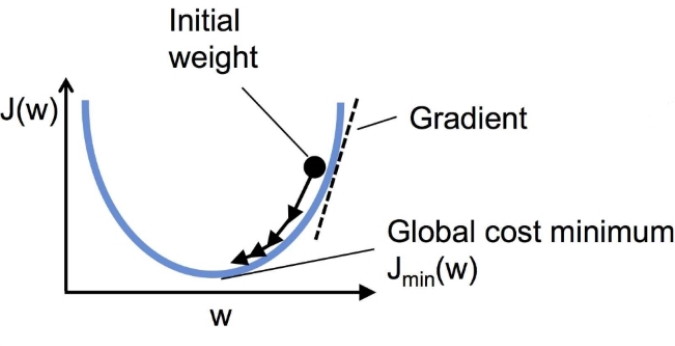
\includegraphics[width=\columnwidth,trim=1 1 1 1,clip]{img/grad_desc_lr_good.png}
            \caption{Well-selected learning rate}
            \label{fig:grad_desc_lr_good}
        \end{subfigure}
        ~ %add desired spacing between images, e. g. ~, \quad, \qquad, \hfill etc.
        %(or a blank line to force the subfigure onto a new line)
        \begin{subfigure}[t]{.33\textwidth}
            \centering
            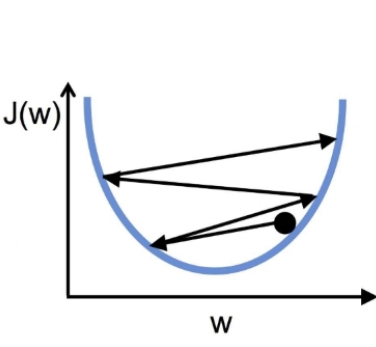
\includegraphics[width=\columnwidth,trim=1 1 1 1,clip]{img/grad_desc_lr_large.png}
            \caption{Learning rate too large}
            \label{fig:grad_desc_lr_large}
        \end{subfigure}
        \caption{If the selected learning rate $\eta$ is too large, instead of minimizing the cost function, the error becomes larger in every epoch, because we overshoot the global minimum.}
        \label{fig:grad_desc_learn_rate}
    \end{figure}

    \subsection{Improving gradient descent through feature scaling} \label{subsec:grad_desc_norm}

    Many machine learning algorithms require some sort of feature scaling for optimal performance.
    Gradient descent is one of the many algorithms that benefit from feature scaling.
    One of the feature scaling methods that can be used is called standardization.
    Standardization gives our data the property of a standard normal distribution, which helps gradient descent learning to converge more quickly.
    Standardization shifts the mean of each feature so that it is centered at zero and each feature has a standard deviation of 1.
    For instance, to standardize the $j^{th}$ feature, we can simply subtract the sample mean $\mu_j$ from every training sample and divide it by its standard deviation $\sigma_j$:

    \begin{equation}
        \label{eq:standardization}
        \large{ \vect{x'}_j = \frac{\vect{x}_j - \mu_j} {\sigma_j} }
    \end{equation}


    Here, $\vect{x}_j$ is a vector consisting of the $^{jth}$ feature values of all training samples n, and this standardization technique is applied to each feature j in our dataset.

    One of the reasons why standardization helps with gradient descent learning is that the optimizer has to go through fewer steps to find a good or optimal solution (the global cost minimum), as illustrated in the figure~\ref{fig:standardization}, where the subfigures represent the cost surface as a function of two model weights in a two-dimensional classification problem.

    \begin{figure}[hbt!]
        \centering
        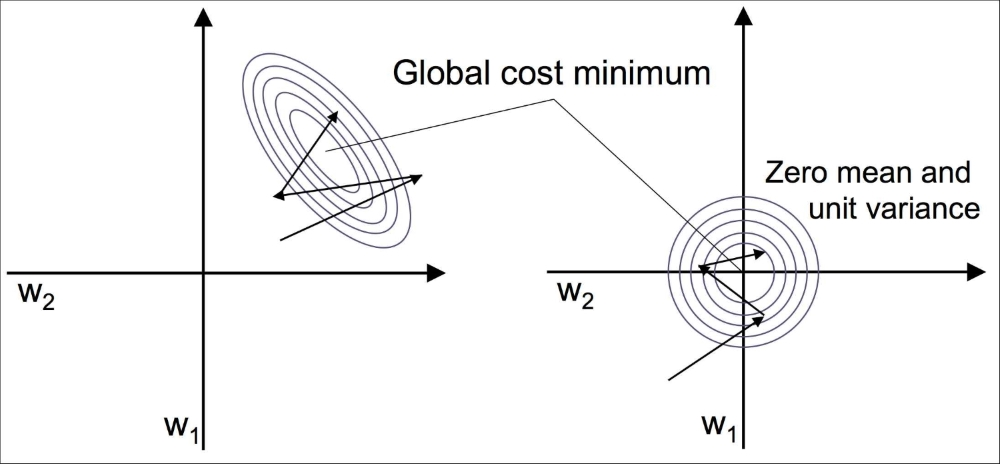
\includegraphics[width=1\linewidth,trim=4 4 4 4,clip]{img/standardization.jpg}
        \caption{Cost surface as a function of two model weights in a two-dimensional classification problem.
        Standardization helps with gradient descent learning because the optimizer has to go through fewer steps to find a good or optimal solution (the global cost minimum)}
        \label{fig:standardization}
    \end{figure}

    Standardization can easily be achieved using the built-in \texttt{NumPy} methods \texttt{mean} and \texttt{std}.

    \section{Training Adaline model on two classes from the Iris dataset} \label{sec:ada_iris}

    After standardization, we will train Adaline again and see that it now converges after a small number of epochs using a learning rate $\eta=0.01$:

    To test the Adaline implementation, Iris flower dataset for classification was used (presented in table~\ref{tab:iris}), from which two flower classes Setosa and Versicolor were loaded.
    Although the Adaline rule is not restricted to two dimensions, only two features were considered (\texttt{sepal length} and \texttt{petal length} for visualization purposes.
    Though only the two flower classes Setosa and Versicolor were chosen for practical reasons, the Adaline algorithm can be extended to multi-class classification \textemdash for example, the \textbf{One-versus-All (OvA)} technique.

    \begin{table}[h!]
        \centering
        \begin{tabular}{||c | c c c c | c||}
            \hline
            index & 0 & 1 & 2 & 3 & 4 \\
            \hline
            \hline
            0 & 5.1 & 3.5 & 1.4 & 0.2 & Iris-setosa \\
            \hline
            1 & 4.9 & 3.0 & 1.4 & 0.2 & Iris-setosa \\
            \hline
            2 & 4.7 & 3.2 & 1.3 & 0.2 & Iris-setosa \\
            \hline
            3 & 4.6 & 3.1 & 1.5 & 0.2 & Iris-setosa \\
            \hline
            4 & 5.0 & 3.6 & 1.4 & 0.2 & Iris-setosa \\
            \hline
        \end{tabular}
        \caption{The first 5 rows from the Iris flower dataset for classification.
        The four features include \texttt{petal\_width}, \texttt{petal\_length}, \texttt{sepal\_width}, and \texttt{sepal\_length}.
        The three class labels are \texttt{Iris-setosa}, \texttt{Iris-versicolor}, and \texttt{Iris-virginica}.}
        \label{tab:iris}

    \end{table}

    First, the first 100 class labels that correspond to the 50 \texttt{Iris-setosa} and 50 \texttt{Iris-versicolor} flowers were extracted, and the class labels were converted into the two integer class labels \texttt{1} (\texttt{versicolor}) and \texttt{-1} (\texttt{setosa}) that we assign to a vector \texttt{y}, where the values method of a \texttt{pandas DataFrame} yields the corresponding \texttt{NumPy} representation.
    In this two-dimensional feature subspace, a linear decision boundary should be sufficient to separate Setosa from Versicolor flowers.
    Thus, a linear classifier such as Adaline should be able to classify the flowers in this dataset perfectly.

    \subsection{Performance of Adaline on two linearly separable classes} \label{subsec:ada_perf_2class}

    \begin{figure}[hbt!]
        \centering
        \begin{subfigure}[t]{.50\textwidth}
            \centering
            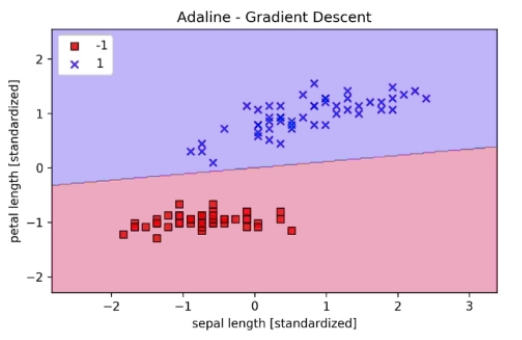
\includegraphics[width=\columnwidth,trim=1 1 1 1,clip]{img/ada_2class_dec.png}
            \caption{Decision boundary}
            \label{fig:ada_2class_dec}
        \end{subfigure}
        ~ %add desired spacing between images, e. g. ~, \quad, \qquad, \hfill etc.
        %(or a blank line to force the subfigure onto a new line)
        \begin{subfigure}[t]{.46\textwidth}
            \centering
            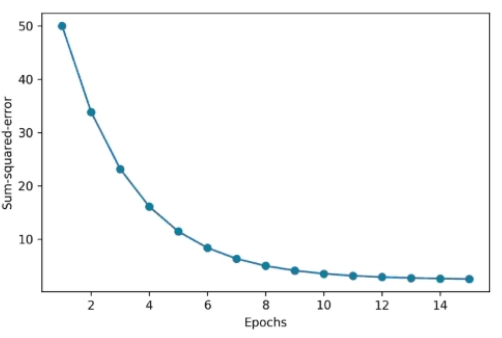
\includegraphics[width=\columnwidth,trim=1 1 1 1,clip]{img/ada_2class_cost.png}
            \caption{Cost per epoch}
            \label{fig:ada_2class_cost}
        \end{subfigure}
        \caption{Decision boundary learned by Adaline and the cost for each epoch.
        Adaline has converged after training on the standardized features using a learning rate $\eta=0.01$.
        However, SSE remains non-zero even though all samples were classified correctly.}
        \label{fig:ada_2class}
    \end{figure}

    Figure~\ref{fig:ada_2class} shows the decision boundary learned by Adaline and the cost for each epoch and can be used to check whether the algorithm converged and found a decision boundary that separates the two Iris flower classes.

    As we can see in the plots, Adaline has now converged after training on the standardized features using a learning rate $\eta=0.01$.
    However, note that the SSE remains non-zero even though all samples were classified correctly.

    \section{Large-scale machine learning and stochastic gradient descent} \label{sec:ada_sgd}

    In the previous section, a cost function was minimized by taking a step in the opposite direction of a cost gradient that is calculated from the whole training set;
    this is why this approach is sometimes also referred to as \textbf{batch gradient descent}.
    In many machine learning applications, it is not uncommon to have a very large dataset with millions of data points.
    In this case, running batch gradient descent can be computationally quite costly in such scenarios since we need to reevaluate the whole training dataset each time we take one step towards the global minimum.
    Alternatively, weights can be updated on each sample, as is done in stochastic gradient descent, or per mini-batches of samples, as is done in mini-batch gradient descent.

    \subsection{Updating weights for each training sample} \label{subsec:ada_sgd}

    A popular alternative to the batch gradient descent algorithm is \textbf{stochastic gradient descent}, sometimes also called \textbf{iterative} or \textbf{online gradient descent}.
    Instead of updating the weights based on the sum of the accumulated errors over all samples $\vect{x^{(i)}}$:

    \begin{equation}
        \Delta \vect{w} = \eta \sum_i \left( y^{(i)} - \phi \left( z^{(i)} \right) \right) \vect{x}^{(i)}
    \end{equation}

    We update the weights incrementally for each training sample:

    \begin{equation}
        \eta \left( y^{(i)} - \phi \left( z^{(i)} \right) \right) \vect{x}^{(i)}
    \end{equation}

    Although stochastic gradient descent can be considered as an approximation of gradient descent, it typically reaches convergence much faster because of the more frequent weight updates.
    Since each gradient is calculated based on a single training example, the error surface is noisier than in gradient descent, which can also have the advantage that stochastic gradient descent can escape shallow local minima more readily if we are working with nonlinear cost functions.
    To obtain satisfying results via stochastic gradient descent, it is \textbf{important to present it training data in a random order}; also, we want to \textbf{shuffle the training set for every epoch} to prevent cycles.

    \subsection{Adaptive learning rate} \label{subsec:ada_sgd_adl}

    In stochastic gradient descent implementations, the fixed learning rate is often replaced by an adaptive learning rate that decreases over time, for example:

    \begin{equation}
        \label{eq:ada_sgd_adl}
        \large{ \frac{c_1} {\text{[number of iterations]} + c2 } }
    \end{equation}

    Where $c_1$ and $c_2$ are constants.
    We shall note that stochastic gradient descent does not reach the global minimum, but an area very close to it.
    And using an adaptive learning rate, we can achieve further annealing to the cost minimum.

    \subsection{Online learning} \label{subsec:ada_sgd_online}

    Another advantage of stochastic gradient descent is that we can use it for \textbf{online learning}.
    In online learning, our model is trained on the fly as new training data arrives.
    This is especially useful if we are accumulating large amounts of data, for example, customer data in web applications.
    Using online learning, the system can immediately adapt to changes and the training data can be discarded after updating the model if storage space is an issue.

    \subsection{Mini-batch learning} \label{subsec:ada_sgd_minibatch}

    A compromise between batch gradient descent and stochastic gradient descent is so-called \textbf{mini-batch learning}.
    Mini-batch learning can be understood as applying batch gradient descent to smaller subsets of the training data, for example, 32 samples at a time.
    The advantage over batch gradient descent is that convergence is reached faster via mini-batches because of the more frequent weight updates.
    Furthermore, mini-batch learning allows us to replace the `for` loop over the training samples in stochastic gradient descent with vectorized operations, which can further improve the computational efficiency of our learning algorithm.

    \subsection{Implementing stochastic gradient descent in Python} \label{subsec:ada_sgd_python}

    \textit{Raschka and Mirjalili}\cite{RaschkaMirjalili2017} make a few adjustments to modify the Adaline learning rule using gradient descent to update the weights via stochastic gradient descent.
    Inside the \texttt{fit} method, weights are now updated after each training sample.
    Furthermore, we will implement an additional \texttt{partial\_fit} method, which does not reinitialize the weights, for online learning.
    In order to check whether our algorithm converged after training, cost as the average cost of the training samples in each epoch is calculated.
    Additionally, an option to shuffle the training data before each epoch is added to avoid repetitive cycles when we are optimizing the cost function;
    via the \texttt{random\_state} parameter, specification of a random seed is allowed for reproducibility.

    \begin{figure}[hbt!]
        \centering
        \begin{subfigure}[t]{.50\textwidth}
            \centering
            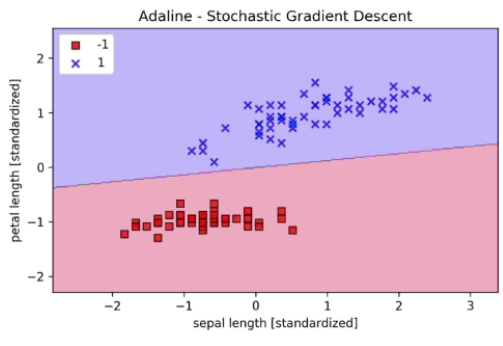
\includegraphics[width=\columnwidth,trim=1 1 1 1,clip]{img/ada_sgd_2class_dec.png}
            \caption{Decision boundary}
            \label{fig:ada_sgd_2class_dec}
        \end{subfigure}
        ~ %add desired spacing between images, e. g. ~, \quad, \qquad, \hfill etc.
        %(or a blank line to force the subfigure onto a new line)
        \begin{subfigure}[t]{.46\textwidth}
            \centering
            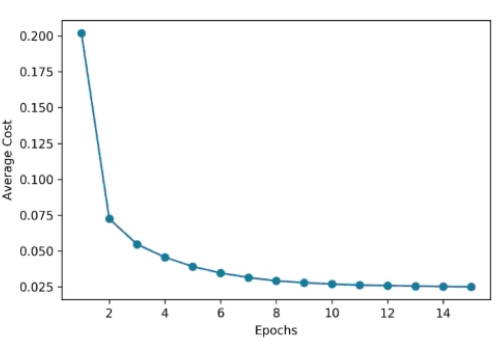
\includegraphics[width=\columnwidth,trim=1 1 1 1,clip]{img/ada_sgd_2class_cost.png}
            \caption{Cost per epoch}
            \label{fig:ada_sgd_2class_cost}
        \end{subfigure}
        \caption{Decision boundary learned by AdalineSGD and the cost for each epoch.
        As we can see, when using stochastic gradient descent, the average cost goes down pretty quickly, and the final decision boundary after 15 epochs looks similar to the batch gradient descent Adaline.}
        \label{fig:ada_sgd_2class}
    \end{figure}

    The \textt{\_shuffle} method that we are now using in the \texttt{AdalineSGD} classifier works as follows: via the \texttt{permutation} function in \texttt{np.random}, a random sequence of unique numbers in the range 0 to 100 is generated.
    Those numbers can then be used as indices to shuffle the feature matrix and class label vector.

    We can then use the \texttt{fit} method to train the \texttt{AdalineSGD} classifier and use our \texttt{plot\_decision\_regions} to plot our training results (shown in figure~\ref{fig:ada_sgd_2class}).

    As we can see, the average cost goes down pretty quickly, and the final decision boundary after 15 epochs looks similar to the batch gradient descent Adaline.
    If we want to update our model, for example, in an online learning scenario with streaming data, we could simply call the \texttt{partial\_fit} method on individual samples \textemdash for instance \texttt{ada.partial\_fit(X\_std[0, :], y[0])}.

    \medskip
    \bibliography{adaline}
    \bibliographystyle{ieeetr}

\end{document}